\begin{frame}{Faces \(\to\) graphs}

We keep only point related to the mouth. 

\bigskip In order to obtain a \textit{weighted graph} from the previous data cloud we opted for two different strategies:

\only<1>{

\begin{itemize}
	\item \textbf{Complete graph} whose vertices are the landmark points of the mouth and  edge-weights $ w_{ij} $ are equal to  the Euclidean distance between vertices $ i $ and $ j $.
\end{itemize}	

\bigskip\centering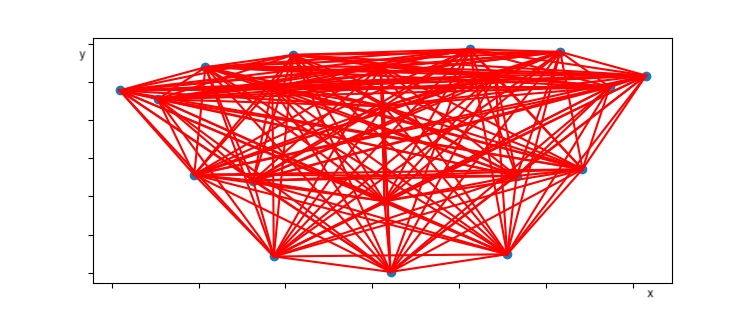
\includegraphics[width=0.5\textwidth]{img/lec5f/boccacomplete.png}}

\only<2>{

\begin{itemize}
	\item \textbf{Meshed graph} obtained using  the Delaunay triangulation algorithm of the  mouth  landmark points (complexity $ O(n \log n) $), also in this case the   edge-weights $ w_{ij} $ are equal to  the Euclidean distance between vertices $ i $ and $ j $.
\end{itemize}	

\bigskip\centering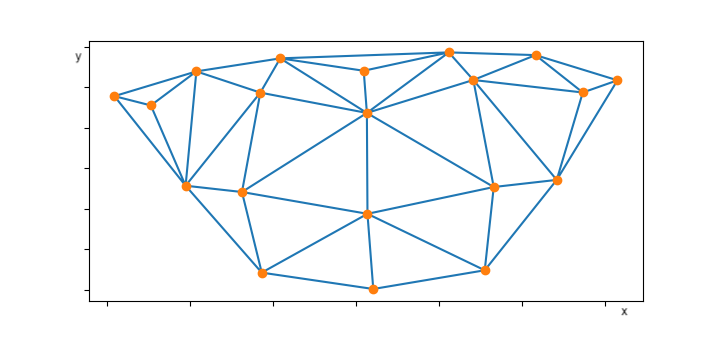
\includegraphics[width=0.5\textwidth]{img/lec5f/boccamesh.png}}

\end{frame}

\begin{frame}{Graph representation}

The graph is represented through its adjacency matrix.

\bigskip We keep only the upper triangular without diagonal, since the graph is undirected (symmetric matrix) and without self loop (the distance between any point with itself is zero). 

\bigskip Vectorize the matrix.

\end{frame}